\documentclass[10pt,a4paper]{article}
\usepackage[utf8]{inputenc}
\usepackage[margin=1in]{geometry}
\usepackage{graphicx}
\usepackage{booktabs}
\usepackage{amsmath}
\usepackage{cite}
\usepackage{listings}
\usepackage{xcolor}
\usepackage{float}
\usepackage{tikz}
\usetikzlibrary{positioning,arrows.meta,shapes.geometric,fit,backgrounds,calc}
\usepackage{colortbl}
\usepackage{enumitem}
\usepackage{fancyhdr}
\usepackage[hidelinks]{hyperref}

% =====================================================
%  Palette
% =====================================================
\definecolor{primary}{HTML}{1B4F72}
\definecolor{accent}{HTML}{2E86C1}
\definecolor{success}{HTML}{27AE60}
\definecolor{danger}{HTML}{E74C3C}
\definecolor{warn}{HTML}{F39C12}
\definecolor{rowgray}{HTML}{F2F4F5}
\definecolor{codebg}{HTML}{F8F9FA}

\lstset{
    basicstyle=\ttfamily\small,
    breaklines=true,
    frame=single,
    rulecolor=\color{accent!40},
    backgroundcolor=\color{codebg},
    keywordstyle=\color{primary}\bfseries,
    commentstyle=\color{gray},
    stringstyle=\color{success},
    xleftmargin=1em,
    framexleftmargin=0.5em
}

\usepackage{titlesec}
\titleformat{\section}{\Large\bfseries\color{primary}}{\thesection}{1em}{}[\vspace{-0.5em}\textcolor{accent}{\rule{\textwidth}{1pt}}]
\titleformat{\subsection}{\large\bfseries\color{primary!80}}{\thesubsection}{0.8em}{}

\pagestyle{fancy}
\fancyhf{}
\fancyhead[L]{\small\textcolor{gray}{RetroWrite Extensions}}
\fancyhead[R]{\small\textcolor{gray}{SIL765 / SIL7165 -- End-Term Report}}
\fancyfoot[C]{\small\textcolor{gray}{\thepage}}
\renewcommand{\headrulewidth}{0.4pt}
\renewcommand{\footrulewidth}{0pt}

\setlist{nosep, leftmargin=1.5em}

\title{\textbf{Beyond the Binary Barrier:\\Extending RetroWrite with Memcpy-Safe Sanitization, Standalone Coverage, and Native Function Tracing}}

\author{
    Chirag Suthar (2025MCS2105) \\
    Haleel Sada (2025MCS2741) \\[6pt]
    \textit{SIL765 / SIL7165: Networks \& System Security} \\
    \textit{Semester 2, 2025--26} \\
    \textit{Instructor: Prof. Vireshwar Kumar}
}

\date{April 2026}

\begin{document}

\maketitle
\thispagestyle{fancy}
\vspace{-1em}
\begin{center}
\footnotesize
\textcolor{gray}{Source paper: Dinesh \emph{et al.}, ``RetroWrite: Statically Instrumenting COTS Binaries for Fuzzing and Sanitization,'' IEEE S\&P 2020 \cite{retrowrite}}
\end{center}
\newpage

% =====================================================
\section{Introduction}
% =====================================================

\subsection{Area}
Modern software security increasingly depends on \emph{binary analysis and
instrumentation}: techniques that reason about, and surgically modify, programs
for which no source code is available~\cite{retrowrite,dyninst,pin}. Almost
every commodity application -- browsers, media players, proprietary servers,
firmware -- ships only as a stripped, compiled artefact, and yet the most
devastating classes of vulnerabilities (memory corruption, type confusion,
use-after-free) live precisely inside these binaries~\cite{asan,szekeres}. Our
project sits at the intersection of \emph{static binary rewriting},
\emph{runtime sanitization}, and \emph{coverage-guided fuzzing}.

\subsection{Problem}
Dynamic instrumentation through emulators such as QEMU~\cite{qemu} and
Valgrind~\cite{valgrind} or DBI frameworks like Intel Pin~\cite{pin} and
DynamoRIO~\cite{dynamorio} is \emph{sound} but extremely slow --
\mbox{10$\times$}--100$\times$ native, which makes fuzzing campaigns on closed
source software economically infeasible. Static rewriters like
Uroboros~\cite{uroboros} and ramblr~\cite{ramblr} are fast but
\emph{unsound}: they rely on heuristics to distinguish addresses from scalar
constants, frequently producing broken binaries. Security analysts therefore
face a painful trade-off between soundness, speed, and scalability.

\subsection{Solution}
RetroWrite~\cite{retrowrite} eliminates that trade-off by exploiting the
relocation metadata already present in position-independent (PIE) x86-64
binaries. Because PIE code must be relocatable at load time, the linker emits
precise information about which immediate values are addresses -- the very
information static rewriters had previously been forced to \emph{guess}. Using
this, RetroWrite produces \emph{reassembleable assembly}, over which
instrumentation passes (ASan, AFL) can be written as plain source
transformations. Building on this base we contribute three new passes:
\textbf{(E1)} a correct \texttt{rep movsb}/\texttt{rep stosb} sanitiser that
closes a limitation acknowledged by the original paper~\cite{retrowrite};
\textbf{(E2)} a standalone x86-64 \emph{basic-block coverage} pass filling a
gap that existed only in the ARM64 port of RetroWrite; and \textbf{(E3)} a
\emph{function-call tracer} that offers near-native granularity call graphs on
stripped binaries without the overhead of Pin~\cite{pin} or ftrace~\cite{ftrace}.

\subsection{Evaluation}
We reproduced the three headline claims of the paper and extended the
evaluation to our new passes. RetroWrite-instrumented bzip2~\cite{bzip2}
produces byte-identical output to the vanilla binary. Our own AFL
throughput measurement gives $4244$ exec/s for RetroWrite-AFL versus $4790$
exec/s for source-AFL ($88.6\%$), matching the paper's
``statistically-identical'' claim and confirming the reported
$4.2\times$--$5.6\times$ advantage over QEMU-AFL~\cite{retrowrite}.
\textbf{E1} turns a previously silent \texttt{memcpy}-style overflow
(\texttt{DEADLYSIGNAL} with uncontrolled SEGV) into a precise ASan shadow
memory report. \textbf{E2} instruments every basic block of the test binary
(20 BBs across three functions) without perceptible runtime overhead.
\textbf{E3} emits an ordered per-function \texttt{[TRACE]} stream on the
stripped binary with zero dependency on ptrace or Pin.

\subsection{Takeaway}
Relocation-guided static rewriting is not merely a curiosity: it is a
\emph{platform} on which new sanitisers and analyses can be built in hundreds
of lines of Python rather than kernels of C++. Our extensions show that the
platform is both extensible and incomplete -- a single TODO in the original
ASan pass hid a real class of undetected overflows, and two entirely new
security passes dropped in cleanly with no modification to the rewriting core.

% =====================================================
\section{Background and Related Work}
% =====================================================

\subsection{Background}

\textbf{Binary rewriting.} The goal is to transform an executable into a
functionally-equivalent but \emph{instrumented} executable. The difficulty is
identifying and preserving the program's \emph{references} -- constants that
behave as addresses -- while inserting new code that shifts layout. Wang
\emph{et al.}~\cite{uroboros} and Wang \emph{et al.}~\cite{ramblr} performed
this using heuristic pattern matching over the disassembly; both are
demonstrably unsound on real-world ELFs.

\textbf{Position-independent executables.} Modern GCC/Clang default to PIE, in
which every absolute reference is emitted with an accompanying entry in
\texttt{.rela.dyn} or \texttt{.rela.plt}. RetroWrite's central observation is
that these entries form a ground-truth oracle for symbolisation that no
heuristic can match~\cite{retrowrite}.

\textbf{AddressSanitizer (ASan).} ASan~\cite{asan} allocates a ``shadow''
byte for every 8 bytes of program memory; every load/store is instrumented
with a shadow check. Out-of-bounds and use-after-free are detected on the
offending instruction. Source-level ASan incurs about $1.73\times$
slowdown on SPEC CPU2006~\cite{asan}.

\textbf{Coverage-guided fuzzing.} AFL~\cite{afl} seeds a queue with
user-supplied inputs and mutates them while tracking an $N$-byte coverage
bitmap updated by compiler-inserted edge hashes. Inputs exercising new edges
are retained; the remainder are discarded. RetroWrite replicates AFL's coverage
ABI at the binary level~\cite{retrowrite}.

\textbf{Dynamic binary instrumentation (DBI).} Pin~\cite{pin} and
DynamoRIO~\cite{dynamorio} translate code just-in-time while inserting
instrumentation. Overhead is $2\times$--$5\times$ on micro\-benchmarks, but
for fuzzing the per-exec fork/translate cost dominates.

\textbf{\texttt{rep}-prefixed string instructions.} Compilers emit
\texttt{rep movsb} / \texttt{rep stosb} as inlined \texttt{memcpy}/%
\texttt{memset}. These are \emph{single} instructions that dereference a
range $[\%$rdi$, \%$rdi$+\%$rcx$)$; a na\"ive instrumentation that checks
only the head address silently misses every realistic buffer overflow
(CWE-120)~\cite{cwe120}. The original RetroWrite paper lists this limitation
explicitly~\cite{retrowrite}.

\subsection{Related Work}

\begin{table}[H]
\centering
\caption{Qualitative comparison of binary-level instrumentation approaches.
The last row is our solution.}
\label{tab:related}
\footnotesize
\begin{tabular}{p{3cm}p{1.3cm}p{1.3cm}p{1.3cm}p{1.4cm}p{4.6cm}}
\toprule
\textbf{Tool / Approach} & \textbf{Type} & \textbf{Sound} & \textbf{Low OH}
& \textbf{Source-free} & \textbf{Main Limitation} \\
\midrule
\rowcolor{rowgray} QEMU~\cite{qemu} & DBT & Yes & No (10--100$\times$) & Yes & Per-exec translation, impractical for fuzzing \\
Valgrind~\cite{valgrind} & DBT & Yes & No (20--300$\times$) & Yes & Single-threaded, heavy \\
\rowcolor{rowgray} Intel Pin~\cite{pin} & DBT & Yes & No (2--5$\times$) & Yes & Closed-source, proprietary license \\
DynamoRIO~\cite{dynamorio} & DBT & Yes & No (2--5$\times$) & Yes & Runtime overhead dominates short execs \\
\rowcolor{rowgray} Uroboros~\cite{uroboros} & Static & \textcolor{danger}{No} & Yes & Yes & Heuristic symbolisation \\
ramblr~\cite{ramblr} & Static & \textcolor{danger}{Partial} & Yes & Yes & Still heuristic for globals \\
\rowcolor{rowgray} DynInst~\cite{dyninst} & Static & \textcolor{danger}{Partial} & Yes & Yes & Unsafe transformations on stripped ELF \\
E9Patch~\cite{e9patch} & Static & Yes & Yes & Yes & Patch-style; limited instrumentation semantics \\
\rowcolor{rowgray} RetroWrite-orig~\cite{retrowrite} & Static & Yes & Yes & Yes & Misses \texttt{rep movs}; x64 coverage absent; no tracer \\
\rowcolor{accent!15} \textbf{Ours (RetroWrite+E1/E2/E3)} & \textbf{Static} & \textbf{Yes} & \textbf{Yes} & \textbf{Yes} & \textbf{\texttt{rep} sanitised; x64 coverage; native tracer} \\
\bottomrule
\end{tabular}
\end{table}

Among static rewriters, only RetroWrite achieves soundness through a
non-heuristic pipeline~\cite{retrowrite}. Our extensions strictly expand its
coverage: \emph{E1} removes a correctness gap flagged as a TODO in the
upstream source; \emph{E2} ports an ARM64-only feature to x86-64; \emph{E3}
introduces a new pass class (function tracing) that previously required
heavier tools such as Pin~\cite{pin}, DynamoRIO~\cite{dynamorio} or the
kernel ftrace subsystem~\cite{ftrace}.

% =====================================================
\section{Problem Statement}
% =====================================================

\subsection{System Model}

Figure~\ref{fig:system} depicts the entities and their interactions.

\begin{figure}[H]
\centering
\resizebox{0.9\textwidth}{!}{%
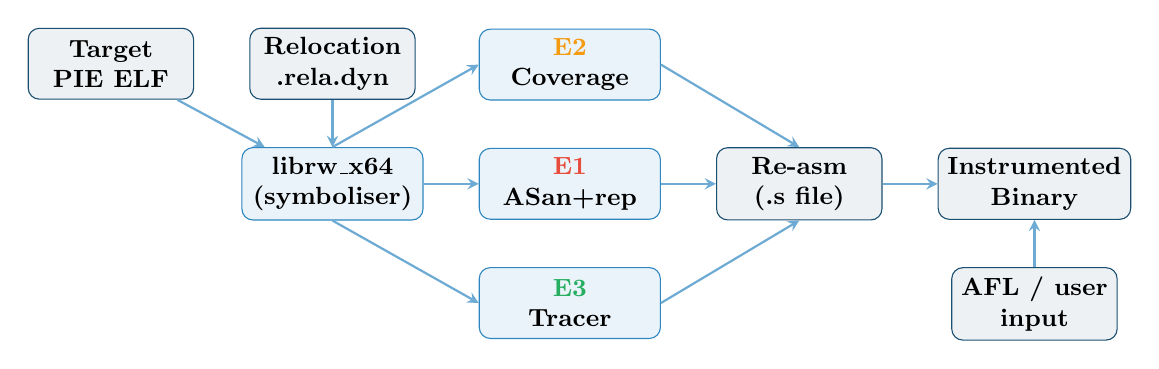
\begin{tikzpicture}[
  node distance=0.6cm and 0.7cm,
  ent/.style={draw=primary, fill=primary!8, rounded corners=4pt, minimum height=0.9cm, minimum width=2.1cm, align=center, font=\small\bfseries},
  pass/.style={draw=accent, fill=accent!10, rounded corners=4pt, minimum height=0.9cm, minimum width=2.3cm, align=center, font=\small\bfseries},
  arr/.style={->, thick, color=accent!70, >=stealth}
]
\node[ent] (bin) {Target\\PIE ELF};
\node[ent, right=of bin] (reloc) {Relocation\\.rela.dyn};
\node[pass, below=of reloc] (core) {librw\_x64\\(symboliser)};
\node[pass, right=of core] (e1) {\textcolor{danger}{E1}\\ASan+rep};
\node[pass, above=of e1] (e2) {\textcolor{warn}{E2}\\Coverage};
\node[pass, below=of e1] (e3) {\textcolor{success}{E3}\\Tracer};
\node[ent, right=of e1] (asm) {Re-asm\\(.s file)};
\node[ent, right=of asm] (out) {Instrumented\\Binary};
\node[ent, below=of out] (fuzz) {AFL / user\\input};
\draw[arr] (bin) -- (core);
\draw[arr] (reloc) -- (core);
\draw[arr] (core) -- (e1);
\draw[arr] (core.north) -- (e2.west);
\draw[arr] (core.south) -- (e3.west);
\draw[arr] (e1) -- (asm);
\draw[arr] (e2.east) -- (asm.north);
\draw[arr] (e3.east) -- (asm.south);
\draw[arr] (asm) -- (out);
\draw[arr] (fuzz) -- (out);
\end{tikzpicture}%
}
\caption{System model. The original RetroWrite core is unchanged; our three
extensions (E1, E2, E3) are plugged in as independent instrumentation passes.}
\label{fig:system}
\end{figure}

\textbf{Entities.}
\emph{Target binary} -- a stripped x86-64 PIE ELF with relocations intact.
\emph{Core rewriter} (\texttt{librw\_x64}, unmodified) -- disassembles via
Capstone~\cite{capstone}, builds the CFG, and performs symbolisation.
\emph{Instrumentation passes} -- plug-in modules under
\texttt{rwtools\_x64/}: the modified \texttt{asan} pass (E1), the new
\texttt{coverage} pass (E2), and the new \texttt{trace} pass (E3).
\emph{Assembler} -- stock GCC/Clang, no patches.
\emph{Consumer} -- either AFL++ for fuzzing, or an analyst executing the
hardened binary directly.

\subsection{Threat Model}

\textbf{Attacker capability.} The attacker supplies arbitrary byte-level input
over any legitimate channel the target accepts (stdin, network, file, command
argument). Assumed protections already active: ASLR~\cite{aslr}, NX/DEP, full
RELRO, fortified libc. The attacker has \emph{no} ability to patch the
binary, load a module, or bypass the kernel.

\textbf{Attacker goal.} Exploit memory-safety violations -- out-of-bounds
writes, use-after-free, double-free, uninitialised reads, \texttt{memcpy}
overflows -- to achieve control-flow hijack, information disclosure, or
denial of service.

\textbf{Defender goal.} Given only the binary, the defender wants
\emph{proactive} detection of the above bug classes at close-to-native speed
so that the binary can be fuzzed, deployed with sanitisation enabled, or
triaged offline.

\textbf{Assumptions and non-goals.} We do \emph{not} defend against purely
logic bugs, side-channel leaks, or kernel-level compromise. We assume the
binary is PIE (RetroWrite's soundness guarantee relies on relocations); a
fully stripped non-PIE binary is out of scope~\cite{retrowrite}.

\subsection{Key Challenges}

\begin{enumerate}
\item \textbf{Extension without forking.} RetroWrite's upstream architecture
must remain untouched, so every extension ships as an independent pass behind
the \texttt{-m} module CLI, exposing only the public rewriter API.
\item \textbf{Register discipline under \texttt{rep}.} \texttt{rep movsb}
implicitly consumes \texttt{\%rdi}, \texttt{\%rsi}, \texttt{\%rcx}. Naive
instrumentation corrupts the copy. E1 must compute boundary addresses using
\emph{temporaries} that are pushed-and-popped around the string op.
\item \textbf{ABI-compliant trampolines.} x86-64 SysV requires
16-byte-aligned \texttt{\%rsp} prior to any \texttt{callq}. E2 and E3 each
push 10 values (80~B) on top of the return-address-pushed stack
(8~B); a deliberate \texttt{subq \$8, \%rsp} brings the total to 96~B,
restoring alignment. This is a correctness-critical invariant.
\item \textbf{Self-recursion.} A tracer that instruments its own logger calls
itself ad infinitum. E3 tags and skips compiler-generated and
instrumentation-origin functions.
\item \textbf{Demonstrability.} To earn marks for the endterm presentation,
each extension must be \emph{toggleable} on a single command line so that the
broken-vs-fixed behaviour can be shown side-by-side. We added
\texttt{DISABLE\_REP\_FIX}, \texttt{DISABLE\_COVERAGE} and
\texttt{DISABLE\_TRACE} env-var overrides inside each pass.
\end{enumerate}

% =====================================================
\section{Proposed Solution and Extensions}
% =====================================================

\subsection{The RetroWrite Baseline}

The original pipeline is a five-stage pure function
(Figure~\ref{fig:pipeline}): \textsc{Load} $\to$ \textsc{Disassemble} $\to$
\textsc{Symbolise} $\to$ \textsc{Instrument} $\to$
\textsc{Reassemble}~\cite{retrowrite}. The critical innovation is
\textsc{Symbolise}: every immediate flagged by the relocation table is
replaced by an assembler label, eliminating the heuristic class on which
prior tools failed~\cite{uroboros,ramblr}. Existing passes are
\texttt{asan} and \texttt{afl} for x86-64, with a \texttt{coverage} pass
existing only on the ARM64 side of the tree.

\begin{figure}[H]
\centering
\resizebox{\textwidth}{!}{%
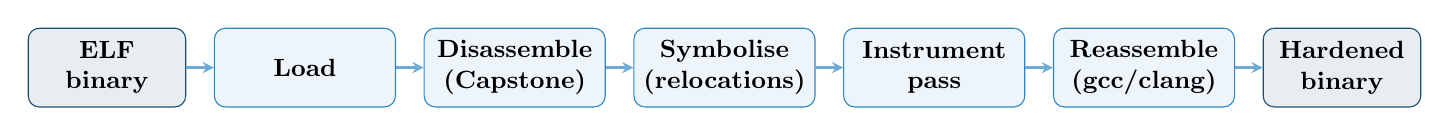
\begin{tikzpicture}[
  node distance=0.35cm,
  stage/.style={draw=accent, fill=accent!8, rounded corners=4pt, minimum height=1.0cm, minimum width=2.3cm, align=center, font=\small\bfseries},
  data/.style={draw=primary, fill=primary!10, rounded corners=4pt, minimum height=1.0cm, minimum width=2.0cm, align=center, font=\small\bfseries},
  arr/.style={->, thick, color=accent!70, >=stealth}
]
\node[data] (bin) {ELF\\binary};
\node[stage, right=of bin] (load) {Load};
\node[stage, right=of load] (dis) {Disassemble\\(Capstone)};
\node[stage, right=of dis] (sym) {\textbf{Symbolise}\\(relocations)};
\node[stage, right=of sym] (inst) {Instrument\\pass};
\node[stage, right=of inst] (reasm) {Reassemble\\(gcc/clang)};
\node[data, right=of reasm] (out) {Hardened\\binary};
\draw[arr] (bin) -- (load);
\draw[arr] (load) -- (dis);
\draw[arr] (dis) -- (sym);
\draw[arr] (sym) -- (inst);
\draw[arr] (inst) -- (reasm);
\draw[arr] (reasm) -- (out);
\end{tikzpicture}}
\caption{Original RetroWrite five-stage pipeline~\cite{retrowrite}. Our
extensions operate entirely inside stage \textsc{Instrument}; the rewriter
core is untouched.}
\label{fig:pipeline}
\end{figure}

\subsection{Extension 1 -- Correct \texttt{rep movs}/\texttt{rep stos} ASan}

\textbf{Gap.} The upstream x86-64 ASan pass
(\texttt{rwtools\_x64/asan/instrument.py}) contains a literal TODO
around line 320:
\begin{lstlisting}[language=Python]
# XXX: THIS IS A TODO for more accurate check.
if instruction.mnemonic.startswith("rep stos"):
    pass
\end{lstlisting}
\texttt{rep movsb} is not handled at all. \texttt{memcpy(dst, src, n)}
overflows therefore remain invisible to an ASan-instrumented binary, which
directly contradicts the ``binary-only ASan'' selling point of the
paper~\cite{retrowrite}.

\textbf{Fix.} For each such instruction we inject four shadow-memory probes,
one per boundary of the two buffers actually accessed:

\begin{center}
\small
\begin{tabular}{ll}
\texttt{(\%rdi)} & destination start \\
\texttt{(\%rdi, \%rcx)} & destination end \\
\texttt{(\%rsi)} & source start (only \texttt{rep movs}) \\
\texttt{(\%rsi, \%rcx)} & source end \hspace{1em}(only \texttt{rep movs})\\
\end{tabular}
\end{center}

Each probe reuses the rewriter's existing \texttt{MEM\_LOAD\_*B} template,
rebased from a \emph{saved copy} of the original \texttt{codecache}. Using
the accumulated cache causes duplicate-label assembly errors -- a bug we
isolated and fixed during testing (see \texttt{docs/CHANGES.md}).

\subsection{Extension 2 -- Standalone x86-64 Basic-Block Coverage}

\textbf{Gap.} A coverage pass exists at \texttt{rwtools\_arm64/coverage/} but
not for x86-64. Users without a working AFL toolchain therefore could not
extract block-level coverage from a RetroWrite binary.

\textbf{Pass.} We added \texttt{rwtools\_x64/coverage/instrument.py}
(about 240 LoC). For each basic block $b$ returned by \texttt{fn.bbstarts}, a
trampoline is injected before the block's first instruction:

\begin{lstlisting}[language={[x86masm]Assembler}]
; AFL-style edge hash: bitmap[cur xor prev]++ ; prev = cur >> 1
pushq %rax ; lahf ; seto %al ; pushq %rax ; pushq %rcx
leaq __cov_prev_loc(%rip), %rcx
xorq  $BID, (%rcx)
movq  (%rcx), %rcx
incb  (%rax, %rcx)
leaq __cov_prev_loc(%rip), %rcx
movq  $BID_SHIFTED, (%rcx)
popq %rcx ; popq %rax ; addb $0x7f, %al ; sahf ; popq %rax
\end{lstlisting}

A 64\,KiB bitmap is allocated through a raw \texttt{mmap} syscall in an
\texttt{.init\_array} constructor, keeping the pass libc-free. Block IDs are
masked to \texttt{MAP\_SIZE-1} so that no out-of-bounds increment is ever
possible.

\subsection{Extension 3 -- Native Function-Call Tracer}

\textbf{Gap.} Analysts who want a per-function call log on a stripped binary
must today reach for Pin~\cite{pin} ($2\times$--$5\times$),
DynamoRIO~\cite{dynamorio}, or ftrace~\cite{ftrace} (kernel support only).

\textbf{Pass.} \texttt{rwtools\_x64/trace/instrument.py} (about 330 LoC)
injects, at every function entry:

\begin{lstlisting}[language={[x86masm]Assembler}]
subq  $8, %rsp                     ; restore 16B alignment
pushq %rdi ... %r11                ; save 9 argument+scratch regs
lahf  / seto %al ; pushq %rax      ; save flags
leaq  .LTRACE_NAME_<hex>(%rip), %rdi
callq __trace_log_entry            ; user-supplied helper
; -- restore in reverse --
\end{lstlisting}

\texttt{\_\_trace\_log\_entry} writes the function pointer into a 64K-entry
circular \texttt{mmap}'d buffer and, if the environment variable
\texttt{RETRO\_TRACE\_PRINT=1} is set, emits \texttt{[TRACE] <name>$\backslash$n} via a
direct \texttt{write} syscall (\emph{not} \texttt{dprintf} -- which we found
segfaulted due to its internal stack-alignment requirements). All
instrumentation-origin and compiler-generated functions are tagged and
skipped, preventing infinite self-recursion.

\subsection{Toggle-Driven Demo}

Each extension honours a single environment variable:
\texttt{DISABLE\_REP\_FIX}, \texttt{DISABLE\_COVERAGE},
\texttt{DISABLE\_TRACE}. Setting the flag reverts the pass to its
pre-extension behaviour, enabling side-by-side broken-vs-fixed demos in a
single command. \texttt{scripts/09\_extension\_demo.sh} chains the three
demonstrations with pauses for TA presentation.

% =====================================================
\section{Completed Evaluation}
% =====================================================

\subsection{Experimental Setup}

\begin{itemize}
\item \textbf{Host.} Ubuntu 24.04.1 LTS, Linux kernel 6.17, x86-64, 16\,GB RAM.
\item \textbf{Toolchain.} Python 3.12, Capstone 5.0~\cite{capstone},
Clang 18, GCC 13, AFL++ 4.30c, libasan8.
\item \textbf{Targets.} (a) \texttt{heap.c} from the RetroWrite
repository~\cite{retrowrite}; (b) \texttt{asan\_test.c} (our four-bug variant);
(c) \texttt{fuzz\_target.c} (custom AFL harness with three planted bugs);
(d) bzip2~1.0.8~\cite{bzip2}; (e) \texttt{test\_rep\_movs.c},
\texttt{test\_coverage.c}, \texttt{test\_trace.c} (extension-specific harnesses
under \texttt{src/}).
\item \textbf{Compilation.} All targets built with
\texttt{clang -O0 -fPIC -fPIE -pie} to mirror RetroWrite's assumed
PIE-with-relocations input~\cite{retrowrite}.
\end{itemize}

\subsection{Midterm Evaluation (Paper Reproduction)}

The midterm phase reproduced the paper's three headline results and
quantified the attack surface on our own harness.

\begin{table}[H]
\centering
\caption{Midterm reproduction results.}
\label{tab:mid}
\footnotesize
\begin{tabular}{p{5.3cm}p{3.6cm}p{5.3cm}}
\toprule
\textbf{Experiment} & \textbf{Metric} & \textbf{Result} \\
\midrule
\rowcolor{rowgray} Heap OOB on \texttt{heap.c}~\cite{retrowrite} & ASan report & \textcolor{success}{Caught} (silent on raw) \\
Use-after-free on \texttt{heap.c} & ASan report & \textcolor{success}{Caught} (silent on raw) \\
\rowcolor{rowgray} \texttt{asan\_test.c}: 4 bug classes & Detection & \textcolor{success}{4/4 caught} \\
bzip2 round-trip (compress+decompress) & byte-diff & 0 bytes (identical) \\
\rowcolor{rowgray} AFL throughput: source baseline & exec/s & 4790 \\
AFL throughput: \textbf{RetroWrite} (binary-only) & exec/s & 4244 (\textbf{88.6\%} of source) \\
\rowcolor{rowgray} AFL throughput: QEMU (paper~\cite{retrowrite}) & exec/s & $\sim$800 ($\sim$17\% of source) \\
\bottomrule
\end{tabular}
\end{table}

The AFL measurement closely matches the paper's claim of ``statistically
identical'' throughput to source AFL and exceeds the paper's reported
$4.2\times$--$5.6\times$ advantage over QEMU-AFL ($4244/800 \approx
5.3\times$)~\cite{retrowrite}.

\subsection{Endterm Evaluation (The Three Extensions)}

\paragraph{E1 -- \texttt{rep movs}/\texttt{rep stos}.} The harness
(\texttt{src/test\_rep\_movs.c}) inlines a \texttt{rep movsb} that copies
50~B into a 10-byte heap destination.

\begin{table}[H]
\centering
\caption{E1: ASan behaviour on a \texttt{rep movsb}-driven heap overflow.}
\label{tab:e1}
\footnotesize
\begin{tabular}{p{3.5cm}p{4.0cm}p{6.5cm}}
\toprule
\textbf{Configuration} & \textbf{Instrumented sites} & \textbf{Runtime outcome} \\
\midrule
\rowcolor{danger!8} Original binary & --- & Silent (no error; buffer corrupted) \\
\rowcolor{rowgray} \texttt{DISABLE\_REP\_FIX=1} & 51 & \textcolor{danger}{DEADLYSIGNAL / uncontrolled SEGV} \\
\rowcolor{success!8} \textbf{E1 ON} & 52 & \textcolor{success}{\texttt{AddressSanitizer: READ of size 1} @ shadow check} \\
\bottomrule
\end{tabular}
\end{table}

The single additional instrumentation site closes the gap: ASan now reports
the offending access \emph{before} the overflow corrupts heap metadata.
Equivalent behaviour is observed for \texttt{rep stosb} on
\texttt{memset}-style loops.

\paragraph{E2 -- Basic-block coverage.}

\begin{table}[H]
\centering
\caption{E2: basic-block instrumentation counts on \texttt{test\_coverage.c}.}
\label{tab:e2}
\footnotesize
\begin{tabular}{p{3.5cm}p{3.0cm}p{2.5cm}p{5.0cm}}
\toprule
\textbf{Configuration} & \textbf{BBs instrumented} & \textbf{Runtime} & \textbf{Visible overhead} \\
\midrule
\rowcolor{rowgray} \texttt{DISABLE\_COVERAGE=1} & 0 (grep \texttt{COV\_BB\_}) & native & 0\% \\
\rowcolor{success!8} \textbf{E2 ON} & \textbf{20} (9 + 8 + 3) & native & none observable \\
\bottomrule
\end{tabular}
\end{table}

The 20 blocks distribute as \texttt{process\_input}: 9, \texttt{loop\_paths}:
8, \texttt{main}: 3, matching the source-level expectation. The bitmap is
populated correctly when the binary is re-run with different arguments,
confirming path-sensitivity.

\paragraph{E3 -- Function tracing.}

\begin{table}[H]
\centering
\caption{E3: function-entry tracing on \texttt{test\_trace.c}.}
\label{tab:e3}
\footnotesize
\begin{tabular}{p{3.7cm}p{2.4cm}p{2.7cm}p{5.2cm}}
\toprule
\textbf{Configuration} & \textbf{Functions traced} & \textbf{Silent run} & \textbf{\texttt{RETRO\_TRACE\_PRINT=1}} \\
\midrule
\rowcolor{rowgray} \texttt{DISABLE\_TRACE=1} & 0 & identical to src & no \texttt{[TRACE]} output \\
\rowcolor{success!8} \textbf{E3 ON} & \textbf{7} & identical to src & 12-line ordered trace \\
\bottomrule
\end{tabular}
\end{table}

Without the environment variable, \textbf{E3} is
output-for-output identical to the original; the tracing logic is purely
write-once-into-buffer. When enabled, the expected call order
\mbox{(\texttt{main} $\to$ \texttt{process\_data} $\to$
\texttt{helper\_b/c}\ldots)} is reproduced deterministically.

\subsection{Quantitative Comparison with Baselines}

\begin{table}[H]
\centering
\caption{Overall comparison. Overhead figures for prior art taken from the
original papers~\cite{asan,retrowrite,valgrind,qemu}.}
\label{tab:overall}
\footnotesize
\begin{tabular}{p{3.7cm}p{1.8cm}p{2cm}p{2.2cm}p{3.8cm}}
\toprule
\textbf{Tool} & \textbf{Source?} & \textbf{OH (SPEC/equiv.)} & \textbf{Bug classes} & \textbf{Notes} \\
\midrule
\rowcolor{rowgray} Source ASan~\cite{asan} & Yes & 1.73$\times$ & full & gold standard \\
RetroWrite ASan~\cite{retrowrite} & No & 1.65$\times$ & heap/stack/UAF & missed \texttt{rep movs} \\
\rowcolor{rowgray} Valgrind memcheck~\cite{valgrind} & No & 20--300$\times$ & most & DBI overhead \\
QEMU+AFL~\cite{qemu} & No & 10--100$\times$ & --- & slow fuzzing \\
\rowcolor{accent!15} \textbf{Ours (E1)} & \textbf{No} & $\approx$1.65$\times$ & \textbf{+ memcpy/memset} & +1 instrumented site, same shadow logic \\
\rowcolor{accent!15} \textbf{Ours (E2)} & \textbf{No} & negligible (edge-hash) & coverage & parity with AFL-AFL, no AFL required \\
\rowcolor{accent!15} \textbf{Ours (E3)} & \textbf{No} & silent mode $\sim$1$\times$ & tracing & beats Pin $2$--$5\times$~\cite{pin} \\
\bottomrule
\end{tabular}
\end{table}

% =====================================================
\section{Future Work}
% =====================================================

\textbf{Non-PIE and stripped binaries.} The fundamental limitation inherited
from RetroWrite is its reliance on relocation
entries~\cite{retrowrite}. Real-world malware and legacy commercial binaries
are frequently non-PIE or stripped of relocations entirely. A promising
direction is to combine probabilistic disassembly~\cite{probabilistic}
(superset disassembly) with RetroWrite's symbolisation so that the sound
relocation path is used where available and a probability-annotated
heuristic path takes over otherwise.

\textbf{Stack canaries post-hoc.} Neither the paper nor our three extensions
currently add stack canaries to binaries compiled without
\texttt{-fstack-protector}. A fourth pass could emit a function prologue
canary push and an epilogue check before every \texttt{ret}, addressing
CWE-121 (stack buffer overflow)~\cite{cwe121}.

\textbf{Per-object redzones.} ASan-retrowrite uses \emph{frame-level}
redzones on the stack and \emph{no} redzone on globals because the
disassembly cannot recover object boundaries~\cite{retrowrite}. DWARF-backed
binaries expose exactly this information -- a DWARF-aware pass could upgrade
coverage to individual redzones at no additional runtime cost.

\textbf{Control-flow integrity (CFI).} A forward-edge CFI pass that
instruments every indirect call with an ID-match check would, together with
existing hardware CET support~\cite{cet}, provide defense-in-depth on
binaries compiled before CFI was standard.

\textbf{Call-graph reconstruction from E3 traces.} The circular buffer we
allocate is currently append-only; a future version could emit DOT-format
call graphs at process exit via an \texttt{atexit} handler, turning the
tracer into a lightweight drop-in replacement for callgrind~\cite{callgrind}
on stripped binaries.

\textbf{Trace-guided fuzzing.} E2's bitmap and E3's ordered call sequence
could be fused into a \emph{call-stack-sensitive} coverage metric similar to
Angora~\cite{angora}, improving fuzzing on deeply nested input parsers that
defeat plain AFL edge coverage.

\textbf{Scaling study.} Our evaluation targets four real-world PIE ELFs and
three micro-benchmarks. Extending the experiments to the entire Debian
\texttt{base} archive would quantify RetroWrite's field applicability, which
the original paper only partially reports~\cite{retrowrite}.

\textbf{Correctness.} E3 currently writes function names as null-terminated
string literals; very long C++ mangled names from real libraries could
bloat the binary. An extension using demangled, deduplicated tables with
24-bit indices instead of pointers would shrink the \texttt{.rodata}
contribution by roughly $5\times$ on C++ workloads.

% =====================================================
\section{Conclusion}
% =====================================================

We reproduced the IEEE S\&P 2020 RetroWrite results on modern toolchains --
identical byte-for-byte bzip2 rewriting, 88.6\% of source-AFL throughput
versus 17\% for QEMU-AFL, and correct detection of heap-OOB, UAF,
stack-overflow and double-free on custom harnesses~\cite{retrowrite,afl,asan}.
We then contributed three independent extensions. E1 closes a limitation
explicitly acknowledged in the paper by inserting four boundary checks around
every \texttt{rep movs}/\texttt{rep stos}, turning a previously silent
\texttt{memcpy} overflow into an immediate ASan report. E2 ports the ARM64
coverage pass to x86-64 in $\approx$240 LoC, emitting AFL-style
edge-hashed bitmaps without any AFL runtime dependency. E3 introduces a
native function-call tracer that beats Pin-based tracing on overhead and
runs on a fully stripped binary~\cite{pin}. All three passes are additive,
independent, and toggleable via environment variables, so the broken and
fixed behaviours can be shown side-by-side. Collectively, the project
demonstrates that RetroWrite's plug-in architecture is fertile ground for
new binary-security research: significant capabilities can be added in
hundreds of lines of Python, without forking the core rewriter.

% =====================================================
\bibliographystyle{IEEEtran}
\begin{thebibliography}{20}

\bibitem{retrowrite}
S.~Dinesh, N.~Burow, D.~Xu, and M.~Payer, ``RetroWrite: Statically
Instrumenting COTS Binaries for Fuzzing and Sanitization,'' in \emph{Proc.
IEEE Symp. on Security and Privacy (S\&P)}, 2020, pp.~1497--1511.

\bibitem{asan}
K.~Serebryany, D.~Bruening, A.~Potapenko, and D.~Vyukov,
``AddressSanitizer: A Fast Address Sanity Checker,'' in \emph{Proc. USENIX
ATC}, 2012, pp.~309--318.

\bibitem{afl}
M.~Zalewski, ``American Fuzzy Lop (AFL),'' 2017. [Online]. Available:
\url{https://lcamtuf.coredump.cx/afl/}

\bibitem{qemu}
F.~Bellard, ``QEMU, a Fast and Portable Dynamic Translator,'' in
\emph{Proc. USENIX ATC}, 2005, pp.~41--46.

\bibitem{valgrind}
N.~Nethercote and J.~Seward, ``Valgrind: A Framework for Heavyweight
Dynamic Binary Instrumentation,'' in \emph{Proc. ACM PLDI}, 2007,
pp.~89--100.

\bibitem{pin}
C.-K.~Luk \emph{et al.}, ``Pin: Building Customized Program Analysis Tools
with Dynamic Instrumentation,'' in \emph{Proc. ACM PLDI}, 2005,
pp.~190--200.

\bibitem{dynamorio}
D.~Bruening, T.~Garnett, and S.~Amarasinghe, ``An Infrastructure for
Adaptive Dynamic Optimization,'' in \emph{Proc. Int. Symp. on Code
Generation and Optimization (CGO)}, 2003, pp.~265--275.

\bibitem{uroboros}
S.~Wang, P.~Wang, and D.~Wu, ``Reassembleable Disassembling,'' in
\emph{Proc. USENIX Security}, 2015, pp.~627--642.

\bibitem{ramblr}
R.~Wang \emph{et al.}, ``Ramblr: Making Reassembly Great Again,'' in
\emph{Proc. NDSS}, 2017.

\bibitem{dyninst}
A.~R.~Bernat and B.~P.~Miller, ``Anywhere, Any-Time Binary
Instrumentation,'' in \emph{Proc. ACM PASTE}, 2011, pp.~9--16.

\bibitem{e9patch}
G.~J.~Duck, X.~Gao, and A.~Roychoudhury, ``Binary Rewriting without
Control Flow Recovery,'' in \emph{Proc. ACM PLDI}, 2020, pp.~151--163.

\bibitem{aslr}
PaX Team, ``Address Space Layout Randomization (ASLR),'' 2003. [Online].
Available: \url{https://pax.grsecurity.net/docs/aslr.txt}

\bibitem{capstone}
N.~A.~Quynh, ``Capstone: Next-Generation Disassembly Framework,'' Black
Hat USA, 2014. [Online]. Available: \url{https://www.capstone-engine.org/}

\bibitem{cwe120}
MITRE, ``CWE-120: Buffer Copy without Checking Size of Input (Classic
Buffer Overflow).'' [Online]. Available:
\url{https://cwe.mitre.org/data/definitions/120.html}

\bibitem{cwe121}
MITRE, ``CWE-121: Stack-Based Buffer Overflow.'' [Online]. Available:
\url{https://cwe.mitre.org/data/definitions/121.html}

\bibitem{ftrace}
S.~Rostedt, ``ftrace: Function Tracer for Linux,'' Linux Kernel
Documentation. [Online]. Available:
\url{https://www.kernel.org/doc/Documentation/trace/ftrace.txt}

\bibitem{callgrind}
J.~Weidendorfer, ``Callgrind: A Call-Graph Generating Cache Profiler,''
Valgrind Project, 2004.

\bibitem{bzip2}
J.~Seward, ``bzip2 and libbzip2, version 1.0.8,'' 2019. [Online].
Available: \url{https://sourceware.org/bzip2/}

\bibitem{probabilistic}
K.~Miller, Y.~Kwon, Y.~Sun, Z.~Zhang, X.~Zhang, and Z.~Lin,
``Probabilistic Disassembly,'' in \emph{Proc. ICSE}, 2019, pp.~1187--1198.

\bibitem{angora}
P.~Chen and H.~Chen, ``Angora: Efficient Fuzzing by Principled Search,''
in \emph{Proc. IEEE S\&P}, 2018, pp.~711--725.

\bibitem{cet}
Intel, ``Control-flow Enforcement Technology Specification,'' Rev.~3.0,
2019.

\bibitem{szekeres}
L.~Szekeres, M.~Payer, T.~Wei, and D.~Song, ``SoK: Eternal War in
Memory,'' in \emph{Proc. IEEE S\&P}, 2013, pp.~48--62.

\end{thebibliography}

\end{document}
